\documentclass[border=2pt,beamer]{standalone}

\usepackage{tikz}
\usetikzlibrary{positioning,decorations.pathreplacing,fit}
\usetikzlibrary{decorations.markings,arrows.meta,shapes.arrows,arrows}
\usetikzlibrary{calc}
\usepackage{cancel}

\definecolor{darkgreen}{RGB}{0,128,80}

\providecommand{\Ckey}{C_{\mathrm{key}}}
\providecommand{\runstate}{\alpha}
\providecommand{\st}{\mathsf{st}}
\providecommand{\running}{\mathsf{running}}
\providecommand{\accepted}{\mathsf{accepted}}
\providecommand{\rejected}{\mathsf{rejected}}




\begin{document}


\begin{standaloneframe}

\resizebox{\textwidth}{!}{

\small




\begin{tikzpicture}[
	arrow double line/.style={
		double distance = 20pt,
   		shorten <= 11, 	
   		shorten >= 16,
   		very thick,
	    postaction = {
    		draw = white,
	 	    line width = 20pt,
	 	    shorten <=-.1pt,
	 	    shorten >=-.1pt,	
	    },
	    postaction = {
	    	decorate, 
	    	decoration = {
	    		markings, 
	    		mark=at position 0 with {
	    			\arrow[xshift=26.6pt]{Straight Barb[reversed,length=-1pt 0.7]}
	    		},
	    		mark = at position 1 with {
   	    			\arrow[xshift=10.6pt]{Straight Barb[length=-1pt 0.7]}
   	    		}
	    	}
	    }
	},
	mybrace/.style= {
		decorate, decoration={brace,amplitude=5pt,raise=5pt}, line width=0.7pt
	},
	mybrace mirror/.style= {
			decorate, decoration={brace,amplitude=5pt,raise=5pt,mirror}, line width=0.7pt
	},
	every node/.style={
		font=\bfseries\boldmath
	},
	]

	\def\AtB{3.3}
	\def\BtT{4.5}
	\def\InterMsgSpaceVertical{1.2}
	
	
	\node[align=center] (client) {\large C};
	\node[above=-0.2 of client] (foo) {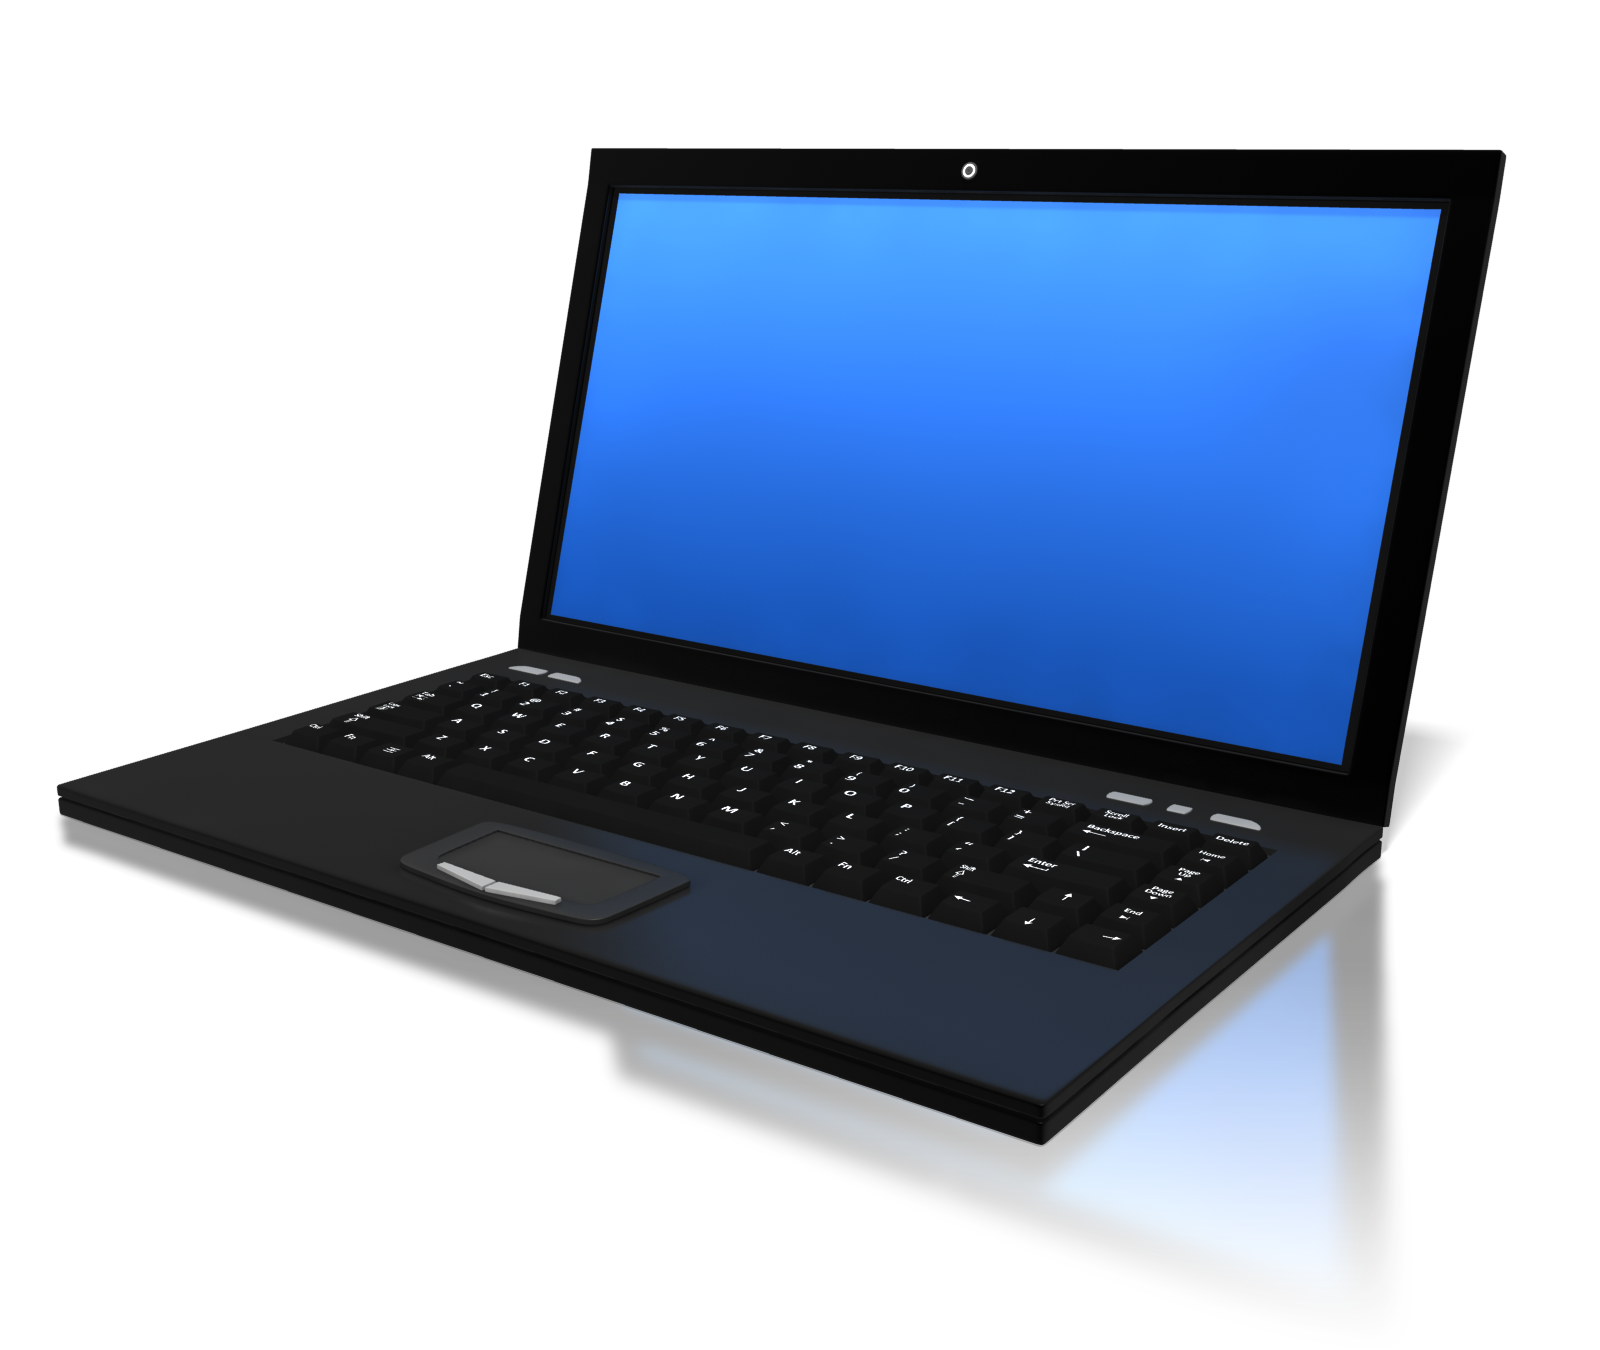
\includegraphics[width=.15\textwidth]{laptop}};
	
	\node[right = \AtB of client,align=center] (AP) {\large A};
	\node[above = 0 of AP] () {
\includegraphics[width=.13\textwidth]{AP}};
	
	\uncover<3-5,8-9>{
		\node[right = 1 of AP,align=center] (AP_Eve) {\large \textbf{B}};
		\node[above = 0 of AP_Eve] () {
\includegraphics[width=.13\textwidth]{AP_black}};
	}
	
	\node[right = \BtT of AP.east,align=center] (AS) {\large S};
	\node[above = -0.2 of AS] () {
\includegraphics[width=.1\textwidth]{server}};
	
	\foreach \i in {1,...,5} {
		\coordinate[below = \InterMsgSpaceVertical * (\i-1) of client] (c\i) {};
		\coordinate[below = \InterMsgSpaceVertical * (\i-1) of AP] (ap\i) {};
		\coordinate[below = \InterMsgSpaceVertical * (\i-1) of AP_Eve] (ap_eve\i) {};
		\coordinate[below = \InterMsgSpaceVertical * (\i-1) of AS] (as\i) {};
	}
	

	\draw[arrow double line,red] (c2) -- node {$\Pi_1$ (2P-AKE), ``C'', {\alt<4-5,8-9>{\xcancel{``A''} \textcolor{black}{\textbf{``B''}}}{``A''}}} (as2);
	
	
	\node[left = 0.05 of c2,align=right] (p1_Ak) {		
		
\includegraphics[width=.06\textwidth]{key_red} 
	};
	
	\node[right = -0.1 of as2,align=left] (p1_Tk) {
		
\includegraphics[width=.06\textwidth]{key_red}
	};


	\visible<7,9-10>{
		\node[left = -0.15 of p1_Ak,align=right] (p1_Ak_w_CB) {
			
\includegraphics[width=.06\textwidth]{key_purple} 
		};
		
		\node[right = -0.1 of p1_Tk,align=left] (p1_Tk_w_CB) {
			{\alt<9>{
\includegraphics[width=.06\textwidth]{key_black}}{
\includegraphics[width=.06\textwidth]{key_purple}}}
		};
	}	
		
	
	\visible<1-3,6-7,10-10>{
		
		\draw[arrow double line, blue] (ap3) -- node {$\Pi_2$ (2P-ACCE)} (as3);
		
		\draw[double,double distance=12, shorten >= 19, shorten <= 11, very thick, blue,
		postaction = {
			draw = white,
			line width = 12pt,
			shorten <= -.1pt,
			shorten >= -.1pt,	
		}] (as4) -- node[yshift=-13,black] {} (ap4);
		
		\draw[-angle 90,shorten >= 8, shorten <= 3,dashed,dash phase=5.3pt, very thick] (as4) -- (ap4);
	
		
		\node[right = -6pt of as4,align=left] (p3_Tk) {
			``C'' \hspace{-6pt} + \hspace{-8pt}   
			{\alt<7,10>{
				
\includegraphics[width=.06\textwidth,trim=0 7cm 0 4cm]{key_purple}
			}{	
				
\includegraphics[width=.06\textwidth,trim=0 7cm 0 4cm]{key_red}
			}}
		};	
		
		\node[left = -11pt of ap4,align=right] (p3_Bk) {
			``C'' \hspace{-6pt} + \hspace{-8pt} 
			{\alt<7,10>{
				
\includegraphics[width=.06\textwidth,trim=0 7cm 0 4cm]{key_purple}
			}{	
				
\includegraphics[width=.06\textwidth,trim=0 7cm 0 4cm]{key_red}
			}}
		};	
	}
	
	
	
	\visible<5-5,8-9>{
		
		\draw[arrow double line, blue] (ap_eve3) -- node {$\Pi_2$ (2P-ACCE)} (as3);
		
		\draw[double,double distance=12, shorten >= 19, shorten <= 9, very thick, blue,
		postaction = {
			draw = white,
			line width = 12pt,
			shorten <= -.1pt,
			shorten >= -.1pt,	
		}] (as4) -- node[yshift=-13,black] {} (ap_eve4);
		
		\draw[-angle 90,shorten >= 9.5, shorten <= 4,dashed, dash phase=0.3pt,very thick] (as4) -- (ap_eve4);
		
		\node[right = -0.19 of as4,align=left] (p3_Tk) {``\textbf{B}''\hspace{-2pt} + 
\includegraphics[width=.06\textwidth,trim=0 7cm 0 4cm]{key_red}};	
				
		\node[left = -9pt of ap_eve4,align=right] (p3_Bk) {``\textbf{B}''\hspace{-2pt} + 
\includegraphics[width=.06\textwidth,trim=0 7cm 0 4cm]{key_red} };
	}
	

	
	\visible<9-9>{
		\node[right = -0.19 of as4,align=left] (p3_Tk) {``\textbf{B}''\hspace{-2pt} + 
\includegraphics[width=.06\textwidth,trim=0 7cm 0 4cm]{key_black}};
		
		\node[left = -9pt of ap_eve4,align=right] (p3_Bk) {``\textbf{B}''\hspace{-2pt} + 
\includegraphics[width=.06\textwidth,trim=0 7cm 0 4cm]{key_black} };
	}
	
	
	\visible<7,10>{	
		\node[draw, below left  = 1.7 and -35pt of as4, align=right,thick, inner sep=4pt] (p1_Tk) {
			$
\includegraphics[width=.06\textwidth, trim=0 7cm 0 4cm]{key_purple} 
			\gets \mathbf{KDF}(
			
\includegraphics[width=.06\textwidth, trim=0 7cm 0 4cm]{key_red}, \text{``C''},\text{``A''})$
		};
	}
	
	\visible<9-9>{	
		\node[draw, below left  = 1.4 and -35pt of as4, align=left,thick, inner sep=4pt] (p1_Tk) {
			$
\includegraphics[width=.06\textwidth, trim=0 7cm 0 4cm]{key_purple} 
				\gets \mathbf{KDF}(
					
\includegraphics[width=.06\textwidth, trim=0 7cm 0 4cm]{key_red},\text{``C''},``\mathbf{A}")$\\
			$
\includegraphics[width=.06\textwidth, trim=0 7cm 0 4cm]{key_black} 
					\gets \mathbf{KDF}(
						
\includegraphics[width=.06\textwidth, trim=0 7cm 0 4cm]{key_red},\text{``C''},\textcolor{black}{``\mathbf{B}"})$
		};
	}
	
	\visible<2,10>{
		\draw[mybrace] ([xshift=1.6cm,yshift=15]as2) -- node[right=0.4,align=center] (3P-KD) {$\Pi_3$} ([xshift=1.6cm,yshift=-13]as4);
	}

\end{tikzpicture}

}

\end{standaloneframe}


\end{document}